\PassOptionsToPackage{dvipsnames,table}{xcolor}
\documentclass[10pt]{beamer}
\usepackage{Cours}

\begin{document}

\input{\detokenize{/home/fenarius/Travail/Cours/NSITerminale/docs/commun/MacrosCours.tex}}
\setcounter{numchap}{8}

\newcommand{\AB}{\cnum Arbres}

\pythonmode


% Vocabulaire sur les arbres
\begin{frame}
	\mframe{\AB}
	\begin{alertblock}{Vocabulaire sur les arbres}
		\begin{itemize}
			\item<1-> Un \textcolor{blue}{arbre} est une structure de données consituée de \textcolor{blue}{noeuds} reliés entre eux par des \textcolor{blue}{arêtes}.
			\item<2-> Contrairement aux listes, piles et files qui sont des structures de données \textbf{linéaires}, les arbres sont des structures de données \textbf{hierarchisées}.
			\item<3-> On dit qu'un noeud B est le \textcolor{blue}{fils} d'un noeud A lorsqu'une arête va du noeud A au noeud B.
			\item<4-> Dans un arbre, un seul et unique noeud n'est le fils de personne, c'est la \textcolor{blue}{racine} de l'arbre.
			\item<5-> Un noeud n'ayant pas de fils s'appelle une \textcolor{blue}{feuille} de l'arbre.
			\item<6-> On appelle \textcolor{blue}{branche} une suite finie de noeuds partant de la racine vers une feuille.
		\end{itemize}
	\end{alertblock}
\end{frame}

% Exemple
\begin{frame}
	\mframe{\AB}
	\begin{exampleblock}{Exemple}
		On représente l'organigramme d'une société par un arbre :
		\begin{center}
			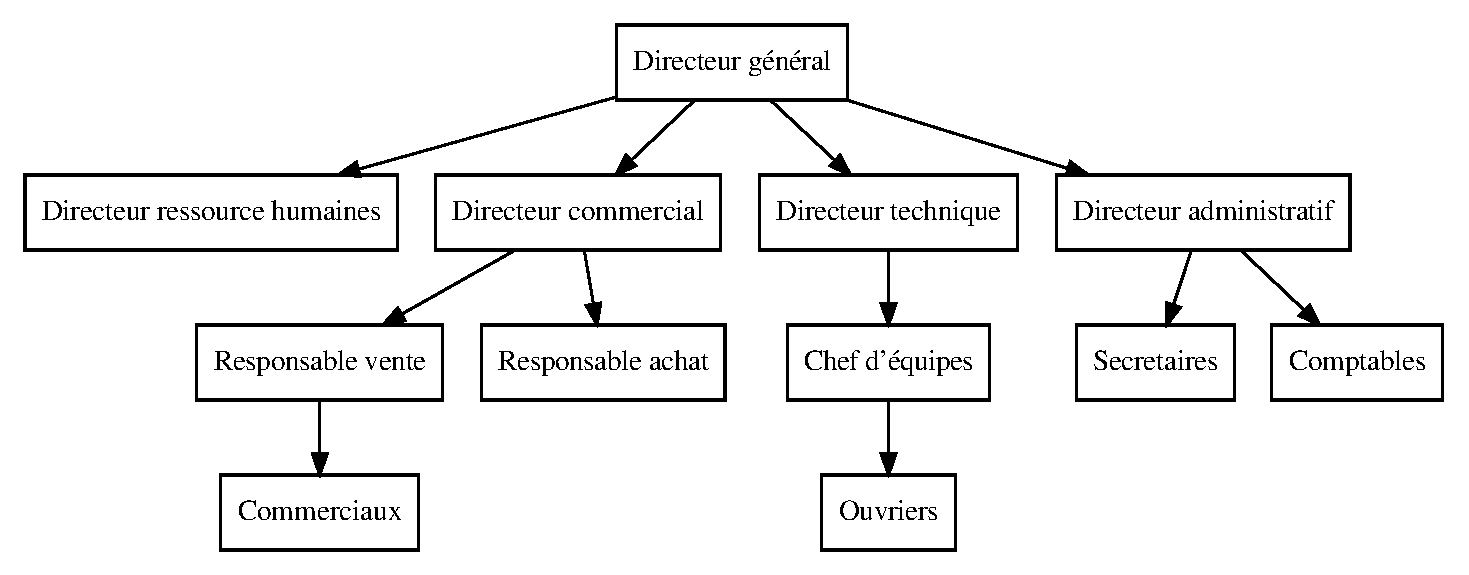
\includegraphics[scale=0.3]{org.gv.eps}
		\end{center}
		\begin{itemize}
			\item<2-> Citer trois noeuds de cet arbre.
			\item<3-> Donner la racine de cet arbre.
			\item<4-> Donner les feuilles de cet arbre.
			\item<5-> Donner une branche de longueur 3 dans cet arbre
		\end{itemize}
	\end{exampleblock}
\end{frame}

% Définiton : taille, arité, hauteur
\begin{frame}
	\mframe{\AB}
	\begin{alertblock}{Définitions}
		\begin{itemize}
			\item<1-> La \textcolor{blue}{taille} d'un arbre est le nombre de noeuds de cet arbre. \\
			      \onslide<2->{\begin{small} \textcolor{gray}{L'arbre vide n'a aucun noeud, sa taille est 0.} \end{small}}
			\item<3-> La \textcolor{blue}{hauteur} d'un arbre est le nombre de noeud maximal qu'une branche peut avoir. \\
			      \onslide<4->{\begin{small} \textcolor{gray}{Différentes définitions existent pour la hauteur d'un arbre, on considère parfois que la hauteur est le nombre maximal d'arête que peut avoir une branche.} \end{small}}
			\item<5-> L'\textcolor{blue}{arité} d'un arbre est le nombre maximal de fils qu'un noeud peut avoir. \\
			      \onslide<6->{\begin{small} \textcolor{gray}{On parle aussi de l'arité (ou degré) d'un noeud, il s'agit alors du nombre de fils de ce noeud} \end{small}}
		\end{itemize}
	\end{alertblock}
	\begin{exampleblock}{Exemple}
		\begin{itemize}
			\item<7-> Quelle est la taille de l'arbre représentant l'organigramme d'une société ci-dessus ?
			\item<8-> Sa hauteur ?
			\item<9-> Son arité ?
		\end{itemize}
	\end{exampleblock}
\end{frame}

% Arbre binaire
\begin{frame}
	\mframe{\AB}
	\begin{alertblock}{Arbre binaire}
		\begin{itemize}
			\item<2->On appelle \textcolor{blue}{arbre binaire} un arbre dans lequel tous les noeuds ont au maximum deux fils. \\
			      \onslide<3->{De façon équivalent, on peut dire qu'un arbre binaire est un arbre d'arité~2.}
			\item<4-> Chaque noeud ayant au plus deux fils, dans un arbre binaire on peut considérer le \textcolor{blue}{sous arbre droit} et le \textcolor{blue}{sous arbre gauche} d'un noeud. Chacun de ces sous arbres étant lui-même un arbre binaire pouvant être vide (noté \textcolor{blue}{$\Delta$}).
			      \onslide<5-> On obtient donc une définition récursive d'un arbre binaire : \\
			      \onslide<6->{Un arbre binaire est soit un arbre vide ($\Delta$) soit un triplet \textit{(noeud,sag,sad)} où \textit{sag} et \textit{sad} sont des arbres binaires.}
		\end{itemize}
	\end{alertblock}
\end{frame}

% Exemple arbre binaire
% Arbre binaire
\begin{frame}
	\mframe{\AB}
	\begin{exampleblock}{Exemple}
		\tei{ab.gv.eps}{0.5}{1}{\begin{itemize}
				\item Vérifier rapidement que cet arbre est binaire.
				\item Compléter l'écriture de cet arbre binaire sous forme de triplet :
				      \begin{itemize}
					      \item (A,sag(A),sad(A))
					      \item (A,(B,sag(B),sad(B)),(C,$\Delta$,$\Delta$))
					      \item \lpo[1]
					      \item \lpo[1]
				      \end{itemize}
				\item Dessiner l'arbre binaire qui s'écrit sous forme de triplet : (A,$\Delta$,(B,(C,(D,$\Delta$,$\Delta$),$\Delta$),(E,$\Delta$,$\Delta$))).
			\end{itemize}}
	\end{exampleblock}
\end{frame}


% Cas particuliers d'arbres binaires
\begin{frame}
	\mframe{\AB}
	\begin{block}{Quelques cas particuliers}
		\begin{itemize}
			\item Un arbre binaire est dit \textit{dégénéré} lorsque tous les noeuds à l'exception des feuilles n'ont qu'un fils. \\
			      \onslide<2->{Exemple d'arbre binaire dégéné de taille 5 :
				      \begin{center}
					      \rnode{A}{\boxed{A}} \qquad \rnode{B}{\boxed{B}} \qquad \rnode{C}{\boxed{C}} \qquad \rnode{D}{\boxed{D}} \qquad \rnode{E}{\boxed{E}} \ncline{->}{A}{B} \ncline{->}{B}{C} \ncline{->}{C}{D} \ncline{->}{D}{E}
				      \end{center} }
			\item<3-> Un arbre binaire est dit \textit{complet} lorsque tous les niveaux sont remplis : \\
			      \onslide<4->{
				      Exemple d'arbre binaire complet de hauteur 3.
				      \begin{center}
					      \begin{tabular}{p{0.3cm}p{0.3cm}p{0.3cm}p{0.3cm}p{0.3cm}p{0.3cm}p{0.3cm}}
						                           &                      &                      & \rnode{A}{\boxed{A}} &                      &                      & \phantom{0}\vspace{0.5cm} \\
						                           & \rnode{B}{\boxed{B}} &                      &                      &                      & \rnode{C}{\boxed{C}} & \phantom{0}\vspace{0.5cm} \\
						      \rnode{D}{\boxed{D}} &                      & \rnode{E}{\boxed{E}} &                      & \rnode{F}{\boxed{F}} &                      & \rnode{G}{\boxed{G}}      \\
						      \ncline{->}{A}{B} \ncline{->}{A}{C} \ncline{->}{B}{D} \ncline{->}{B}{E} \ncline{->}{C}{F} \ncline{->}{C}{G}
					      \end{tabular}
				      \end{center}}
		\end{itemize}
	\end{block}
\end{frame}

% Relation entre hauteur et taille
\begin{frame}
	\mframe{\AB}
	\begin{alertblock}{Relation entre hauteur et taille}
		En notant $n$ la taille et $h$ la hauteur d'un arbre binaire, pour $n \geq 2$, on a la relation suivante : \\
		\onslide<2->{$$ \boxed{ h \leq n \leq 2^{h}-1} $$}
	\end{alertblock}
	\begin{exampleblock}{Exemples}
		\begin{itemize}
			\item<3-> Quelle est la relation entre $h$ et $n$ dans le cas d'un arbre binaire dégénéré ?
			\item<4-> Même question dans le cas d'un arbre binaire complet.
		\end{itemize}
	\end{exampleblock}
\end{frame}


% Relation entre hauteur et taille
\begin{frame}
	\mframe{\AB}
	\begin{alertblock}{Parcours d'un arbre}
		On peut parcourir un arbre binaire :
		\begin{itemize}
			\item<2-> En largeur, cela revient à lister les noeuds par ordre croissant de profondeur et de gauche à droite \\
			      \onslide<3-> \textcolor{gray}{L'implémentation de ce parcours peut se faire à l'aide d'une file dans laquelle on stocke les noeuds restants à parcourir. A chaque fois qu'on traite un noeud, on le defile et on enfile ses fils (voir la fiche d'activité).}
			\item<3-> En profondeur, on tire alors partie de la structure récursive des arbres. Pour parcourir l'arbre $T=(e,sag,sad)$ on doit relancer le parcours sur $sag$ et $sad$. On distingue alors trois parcours suivant que $e$ est affiché avant, entre ou après $sag$ et $sad$ :
			      \begin{itemize}
				      \item<4-> Dans le parcours préfixé, $e$ est affiché avant de parcourir $sag$ et $sad$.
				      \item<5-> Dans le parcours infixé, $e$ est affiché après le parcours de $sag$ mais avant celui de  $sad$.
				      \item<6-> Dans le parcours suffixé, $e$ est affiché après le parcours de $sag$ et $sad$
			      \end{itemize}
		\end{itemize}
	\end{alertblock}
\end{frame}


\begin{frame}
	\mframe{\AB}
	\begin{exampleblock}{Exemple}
		\begin{center}
			\begin{tabular}{p{0.3cm}p{0.3cm}p{0.3cm}p{0.3cm}p{0.3cm}p{0.3cm}p{0.3cm}}
				                     &                      &                      & \rnode{A}{\boxed{R}} &                      &                      & \phantom{0}\vspace{0.5cm} \\
				                     & \rnode{B}{\boxed{T}} &                      &                      &                      & \rnode{C}{\boxed{C}} & \phantom{0}\vspace{0.5cm} \\
				\rnode{D}{\boxed{V}} &                      & \rnode{E}{\boxed{I}} &                      & \rnode{F}{\boxed{F}} &                      & \phantom{0}\vspace{0.5cm} \\
				                     & \rnode{I}{\boxed{M}} &                      & \rnode{G}{\boxed{P}} &                      & \rnode{H}{\boxed{A}} &                           \\
				\ncline{->}{A}{B} \ncline{->}{A}{C} \ncline{->}{B}{D} \ncline{->}{B}{E} \ncline{->}{F}{G} \ncline{->}{F}{H} \ncline{C}{F} \ncline{D}{I}
			\end{tabular}
		\end{center}
		Donner l'ordre des noeuds lorsqu'on parcourt l'arbre ci-dessus :
		\begin{itemize}
			\item<1-> En largeur
			\item<2-> En profondeur préfixé
			\item<3-> En profondeur infixé
			\item<4-> En profondeur suffixé
		\end{itemize}
	\end{exampleblock}
\end{frame}

\begin{frame}
	\mframe{\AB}
	\begin{alertblock}{Arbre binaire de recherche}
		Un arbre binaire \textcolor{blue}{de recherche} (noté {\sc abr}), est un arbre binaire tel que :
		\begin{itemize}
			\item<2-> Les étiquettes des noeuds, appelées \textcolor{blue}{clé} sont toutes comparables entre elles. \\
			      \onslide<4->{\textcolor{gray}{Par exemple, les étiquettes sont toutes des nombres ou encore des chaines de caractères (comparées par ordre alphabétique).}}
			\item<5-> Pour tous les noeuds l'ensemble des clés présentes dans le sous arbre gauche (resp. droit) sont strictement inférieures (resp. supérieures) à la clé du noeud.\\
			      \onslide<6->{\textcolor{gray}{Par souci de simplicité, on admettra que les clés sont uniques dans un {\sc abr} ce qui permet d'éviter le cas de clés égales}}
		\end{itemize}
	\end{alertblock}
\end{frame}

\begin{frame}
	\mframe{\AB}
	\begin{exampleblock}{Exemple}
		\begin{center}
			\begin{tabular}{p{0.3cm}p{0.3cm}p{0.3cm}p{0.3cm}p{0.3cm}p{0.3cm}p{0.3cm}}
				                     &                      &                      & \rnode{A}{\boxed{10}} &                       &                       & \phantom{0}\vspace{0.5cm} \\
				                     & \rnode{B}{\boxed{6}} &                      &                       &                       & \rnode{C}{\boxed{19}} & \phantom{0}\vspace{0.5cm} \\
				\rnode{D}{\boxed{4}} &                      & \rnode{E}{\boxed{?}} &                       & \rnode{F}{\boxed{16}} &                       & \phantom{0}\vspace{0.5cm} \\
				                     & \rnode{I}{\boxed{5}} &                      & \rnode{G}{\boxed{13}} &                       & \rnode{H}{\boxed{17}} &                           \\
				\ncline{->}{A}{B} \ncline{->}{A}{C} \ncline{->}{B}{D} \ncline{->}{B}{E} \ncline{->}{F}{G} \ncline{->}{F}{H} \ncline{C}{F} \ncline{D}{I}
			\end{tabular}
		\end{center}
		\begin{itemize}
			\item<1-> Cet arbre est-il un {\sc abr} si la clé manquante est 2 ? 9 ? 12 ?
			\item<2-> On suppose que la clé manquante est 9. Proposer une nouvelle valeur pour le noeud de clé 16 de façon à ce que cet arbre reste un {\sc abr}.
			\item<3-> Proposer une valeur pour le noeud de clé 16 de façon à ce que cet arbre ne soit pas un {\sc abr}
		\end{itemize}
	\end{exampleblock}
\end{frame}

\begin{frame}
	\mframe{\AB}
	\begin{alertblock}{Recherche dans un {\sc abr}}
		\begin{itemize}
			\item<1-> La recherche d'un élément dans un {\sc abr} a pour complexité la hauteur de cet arbre. En effet, on descend d'un niveau dans l'arbre à chaque étape de la recherche en choisissant d'aller à gauche ou à droite suivante que l'élément recherché est plus petit ou plus grand que le noeud parcouru.
			\item<2-> Par conséquent, si l'arbre est dégénéré, la hauteur est égale au nombre de noeuds et l'algorithme équivaut à la recherche dans une liste.
			\item<3-> Si l'arbre est complet par contre la complexité est logarithmique et équivaut à une recherche dichotomique dans une liste triée.
		\end{itemize}
	\end{alertblock}
\end{frame}

\end{document}